\documentclass[18pt]{article}
\usepackage[utf8]{inputenc}
\usepackage[T1]{fontenc}
\usepackage{ragged2e}
\usepackage{caladea}
\usepackage{graphicx}
\usepackage{longtable}
\usepackage{wrapfig}
\usepackage{rotating}
\usepackage{epigraph}
\usepackage[normalem]{ulem}
\usepackage{hyperref}
\usepackage{amsmath}
\usepackage{amssymb}
\usepackage{capt-of}
\usepackage{hyperref}
\usepackage{fancyhdr}

\title{
 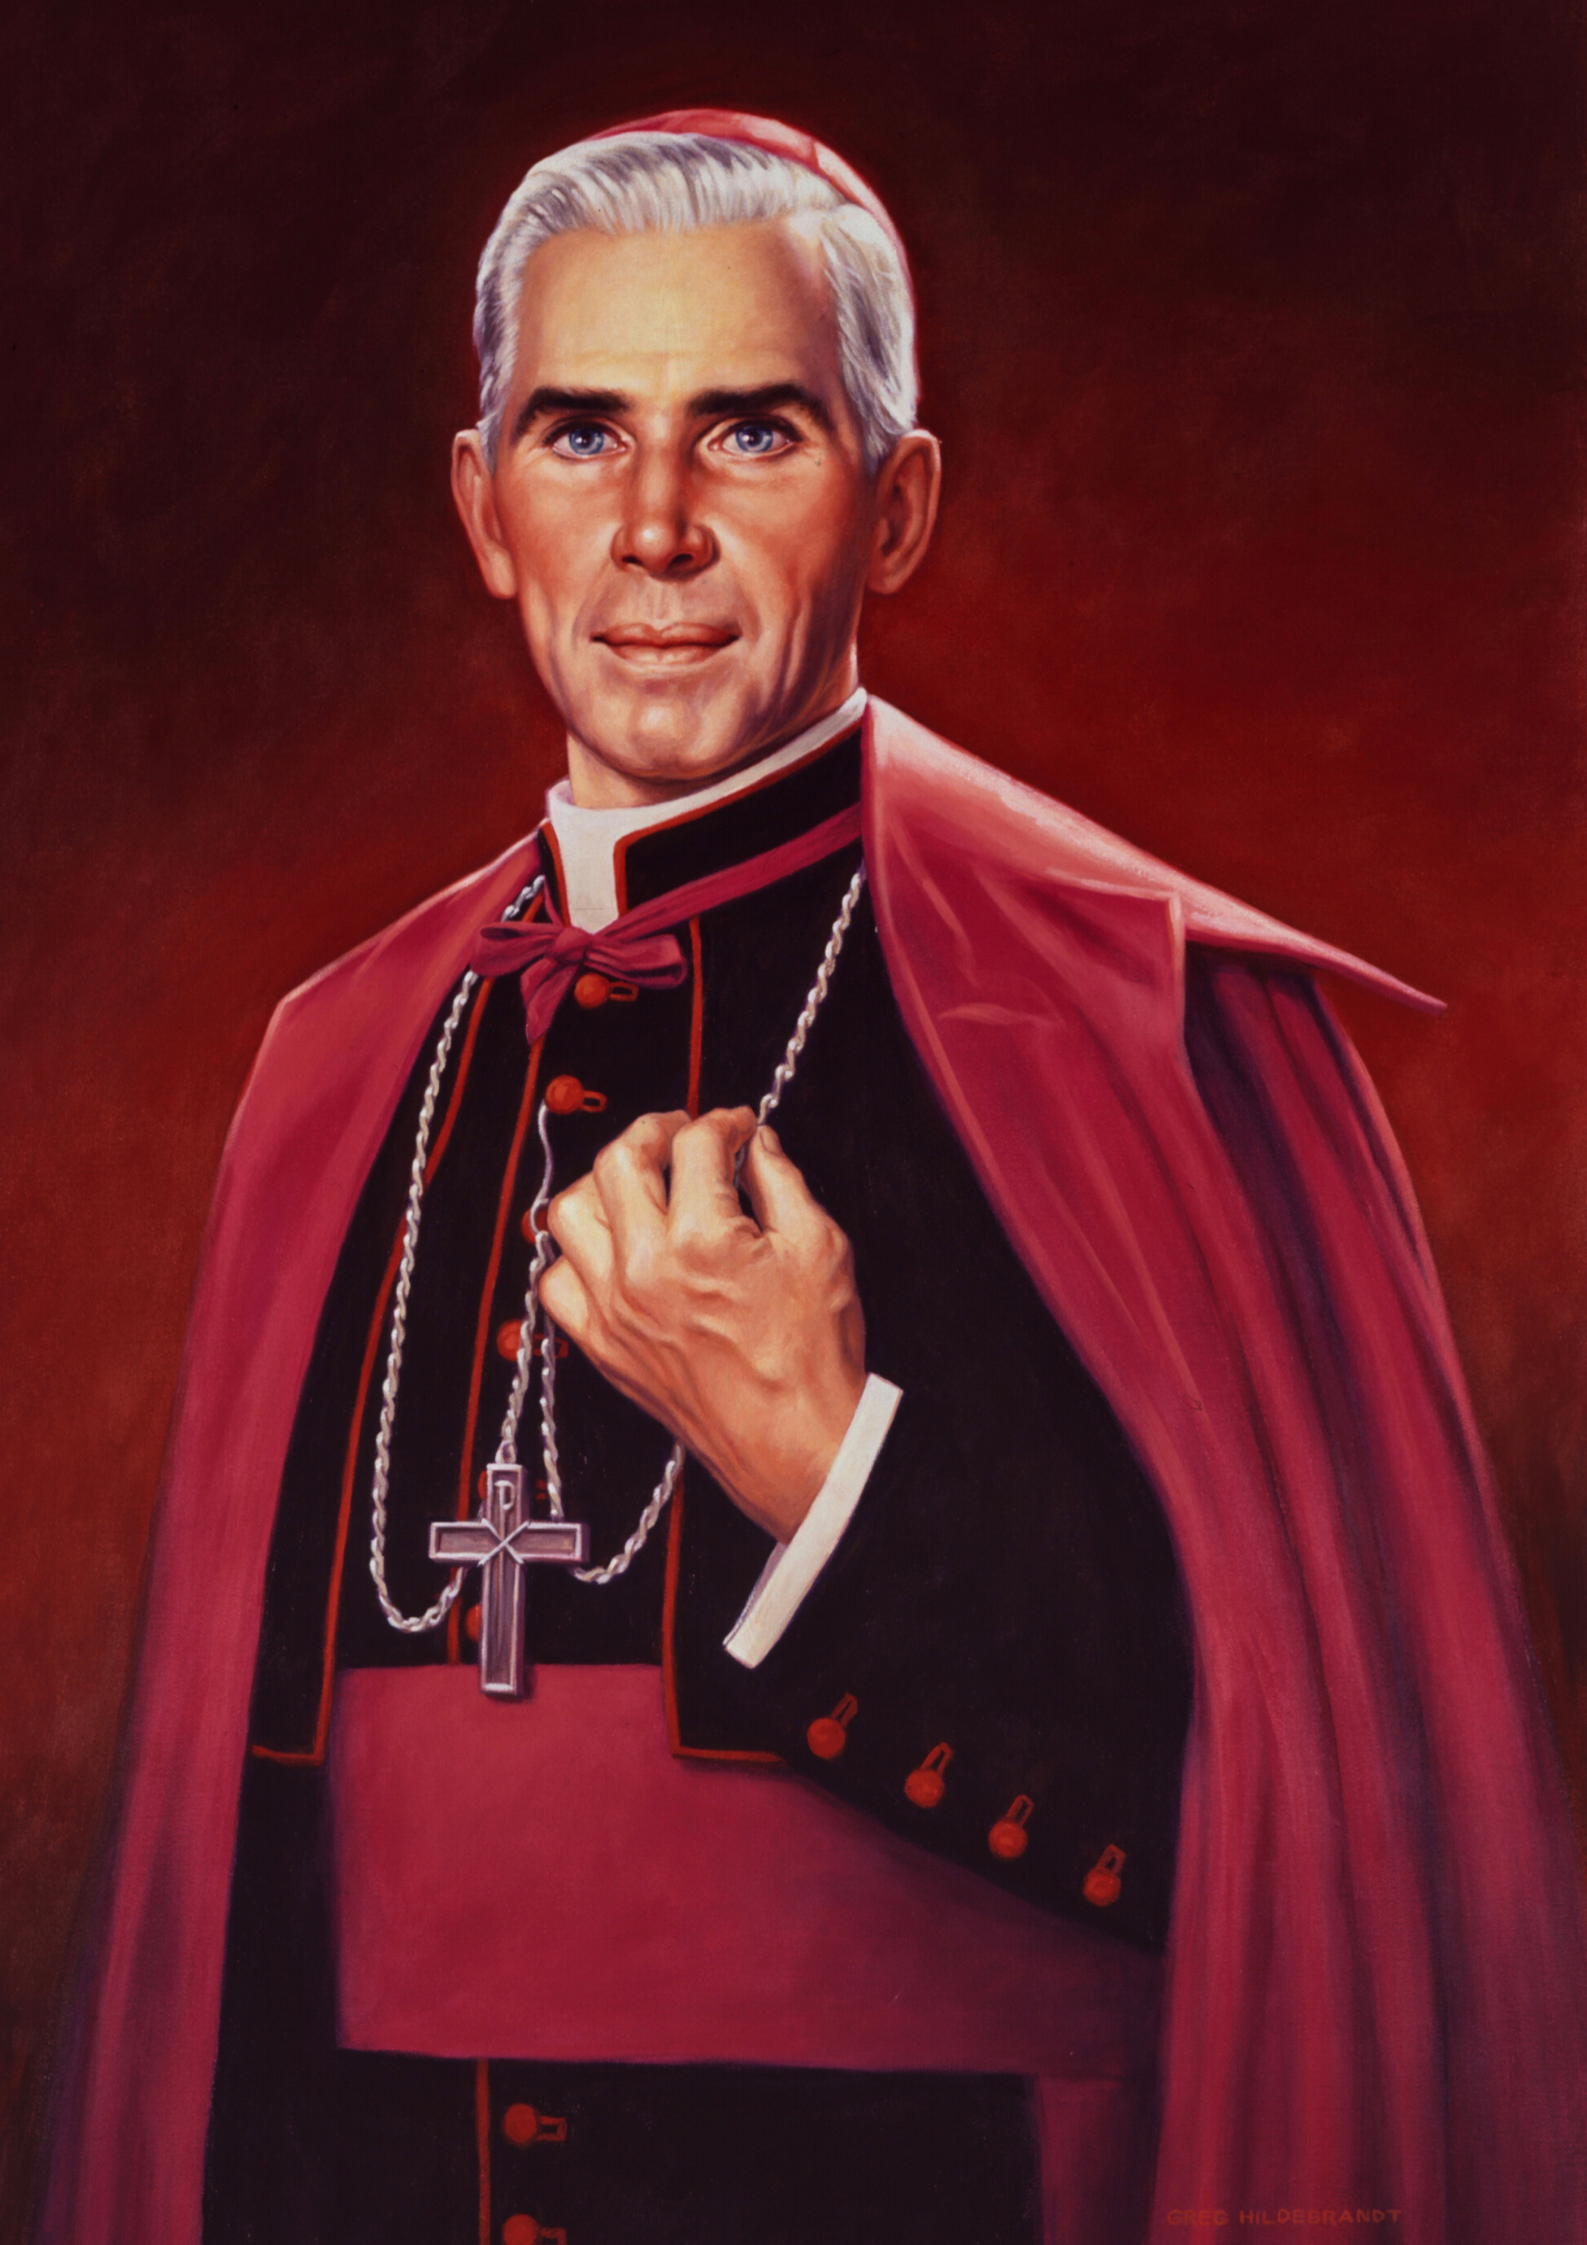
\includegraphics[scale=.55, trim={10cm, 0, 10cm, 0}]{./assets/imagem.jpg}
  \par
   NOVENA A SANTA BERNADETTE SOUBIROUS}
  \date{ Data de Início: 07/04 Data Litúrgica: 16/04}

% Comando para fazer "Sumário" não aparecer no Sumário.
\renewcommand{\contentsname}{Sumário}
\begin{document}
\maketitle

\thispagestyle{empty} %zera a primeira página

\pagestyle{fancy}
\fancyhf{} % clear existing header/footer entries
\fancyfoot[LO, CE]{
\includegraphics[scale=0.2]{./assets/cross.png} Santa Bernadette Soubirous, rogai por nós!
}
% Place Page X of Y on the right-hand
% side of the footer
\fancyfoot[R]{\thepage}

\newpage

\tableofcontents

\centering
\vfill
Visite-nos no Telegram: \url{https://t.me/CotidieNovena}
\newpage

\newpage


%%%%%%%%%%%%%%%%%%%%%%%%%%%%%%%%%%%%% História %%%%%%%%%%%%%%%%%%%%%%%%%%%%%%%%%%%%%%%%%%%

\begin{justify}

 \begin{center}
  \section{História}\label{sec:História} % (fold)
 \end{center}


Santa Bernadette nasceu no moinho de Boly, perto de Lourdes, na França, no dia 7 de janeiro de 1844. Foi a filha mais velha entre 9 filhos de Francisco Soubirous e Luisa Castérot. Seu pai era um pobre moleiro (operário de moinho de farinha) e viviam em condições precárias. Na infância Bernadette foi pastora e doméstica.

Para piorar a situação, a região começou a enfrentar uma grave crise financeira. Por isso, mudaram-se para Lourdes, em condição de miséria. Em Lourdes, vão morar na antiga cadeia que estava abandonada. Este era um lugar sujo e infecto. Assim, Bernadette, que sempre tivera pouca saúde, piorou seu estado sofrendo com cólera e asma. Ela não pode frequentar a escola ficando analfabeta até os 14 anos.


\begin{justify}
\subsection{ Aparições de Nossa Senhora Lourdes a Santa Bernadette }
\end{justify}

No dia 11 de fevereiro de 1858, Bernadette, sua irmã Toinette e a amiga Baloume foram buscar lenha na gruta de Massabielle (rocha velha). Nesse dia Santa Bernadette viu uma mulher de branco, com um rosário na mão e um cinto brilhante. Mais tarde, esta mulher da visão se revelaria como Nossa Senhora da Imaculada Conceição.

No momento da visão Bernadette disse que ficou com medo e começou a rezar o terço. Então seu coração se acalmou e ela teve serenidade para saber que realmente se tratava de uma aparição de Nossa Senhora. A partir desse momento Bernadette teve 18 aparições de Nossa Senhora, ocorridas entre 11 de fevereiro e 16 julho do ano de 1858.


\begin{justify}
\subsection{Uma água milagrosa brota na gruta}
\end{justify}

Na aparição do dia 25 de fevereiro, Nossa Senhora mandou que Bernadette cavasse o chão na gruta Massabielle. Onde ela cavou, brotou uma fonte de água pura que jorra cerca de 5 mil litros por dia até os dias de hoje. Desse dia em diante, milhares de curas extraordinárias já aconteceram a enfermos que se banharam nas águas abençoadas da gruta de Lourdes.


\begin{justify}
\subsection{Nossa Senhora se revela ao mundo}
\end{justify}

Maria pediu a Santa Bernadette que fosse à gruta por 15 dias. Na 16ª aparição, ela revelou como queria ser chamada. Nossa Senhora disse: Eu sou a Imaculada Conceição. O Padre Dominique, pároco local, que conhecia Bernadette, disse que era impossível ela conhecer o Dogma (verdade de fé) da Imaculada Conceição, estabelecido em 1854 pelo Papa Pio lX, 4 anos antes das aparições em Lourdes. Como vimos, Bernadette era analfabeta e de família muito pobre.


\begin{justify}
\subsection{Promessa de Nossa Senhora de Lourdes a Santa Bernadette}
\end{justify}

Em uma das aparições, Nossa Senhora disse a Bernadette: Não prometo fazer-te feliz nesse mundo, mas sim no outro. E, de fato, Bernadette foi submetida a inúmeros interrogatórios, dúvidas e questionamentos por parte de autoridades da Igreja e de céticos. Porém, para espanto e admiração de todos, Bernadette defendeu as aparições de Nossa Senhora com muita força e convicção, sem deixar de lado sua simplicidade e humildade


\begin{justify}
\subsection{Milagres de Nossa Senhora de Lourdes na gruta}
\end{justify}

Numerosos milagres aconteceram na gruta de Lourdes dos dias de Bernadette até hoje.

Uma mulher grávida de 9 meses com uma mão paralítica vai a gruta, vê ali Santa Bernadette tendo uma das visões de Nossa Senhora e depois das orações coloca sua mão paralítica na água da fonte ficando milagrosamente curada.

Muitos milagres acontecem nos dias de hoje no Santuário de Lourdes, que recebe anualmente mais de 6 milhões de peregrinos de todas as partes do mundo.


\begin{justify}
\subsection{Milagres de Santa Bernadette}
\end{justify}

Santa Bernardete realizou muitos milagres em vida e mais ainda após a sua morte. Dois milagres em vida ficaram muito famosos.

Um recém nascido tuberculoso, desenganado pelos médicos, foi levado por sua mãe ao convento que para Santa Bernadette acabar de bordar a roupa do doente, quando sua mãe coloca a roupa no doente ele fica curado.

Uma mãe leva a filha aleijada no convento e pede para Bernadette segurá-la. A superiora diz para que ela não a deixe no chão, mas logo Santa Bernadette a deixa brincar e correr para todos os lados, pois ficou milagrosamente curada.


\begin{justify}
\subsection{Refugio de Santa Bernadette}
\end{justify}

Por causa dos milagres e visões, a fama de Bernadette se espalhou e muitas pessoas vinham procura-la de todas as partes. Para fugir dessa gente, Bernadette se internou no hospital das Irmãs de Caridade em Nevers, Lourdes. Ali, ela recebeu aulas, aprendeu a ler e escrever. Lá ela faz de próprio punho, o primeiro relato das aparições de Lourdes.

Em janeiro de 1862, o Monsenhor Bertrand Séveré Laurence, Bispo de Tarbes, reconheceu oficialmente o relato das aparições.


\begin{justify}
\subsection{Vida Religiosa de Santa Bernadette}
\end{justify}

No convento, Bernadette sentiu confirmada sua vocação para a vida religiosa. Então, ela entra para o convento de Saint Gildad, iniciando seu noviciado em 1866. Em 30 de outubro de 1867, faz a profissão religiosa nas Irmãs da Caridade de Nevers.

Bernadette dedicou sua vida à ajuda aos necessitados como enfermeira. Assim ela se sentia realizada, podendo demonstrar o amor de Deus aos doentes, dando-lhes alento, conforto e esperança. Assim viveu até sua morte.


\begin{justify}
\subsection{Santa Bernadette falece}
\end{justify}

Santa Bernadette sofria de uma doença que a deixou totalmente paralisada em seus últimos anos de vidas. Ela faleceu no dia 19 de abril do ano de 1897, estando totalmente imobilizada na cama.

Com a divulgação da notícia de sua morte, grande multidão foi ao convento prestar suas homenagens e orações a Santa Bernadette. Seu sepultamento teve que ser adiado, para que todos pudessem dar o último adeus a Bernadette.


\begin{justify}
\subsection{Corpo incorrupto de Santa Bernadette}
\end{justify}

Trinta anos após sua morte, seu corpo foi exumado por causa do processo de canonização que se iniciara em seu favor. E, para o espanto de todos, seu corpo estava intacto, incorrupto, do mesmo modo como ela tinha sido enterrada, apesar de seu hábito apresentar humidade e o rosário em suas mãos ter oxidado.

O povo passou a chamar Santa Bernadette de Santa Dormente pois, em seu leito de morte, parece que ela está apenas dormindo. Hoje, mais de um século após sua morte, seu corpo continua intacto e está exposto em uma redoma de vidro, na Igreja do Convento de Saint Gildard de Nevers.


\begin{justify}
\subsection{Canonização}
\end{justify}

Tendo milagres estudados e confirmados pela Igreja, o Papa Pio XI celebrou a canonização de Santa Bernadette de Lourdes no dia 8 de dezembro de 1933, festa da Imaculada Conceição. A santidade de Bernadette foi confirmada ao longo de sua vida no convento.

Todos testemunhavam o amor, a fé, a perseverança e o carinho que Santa Bernadette demonstrava para com todos. Sua festa é celebrada no dia 16 de abril. Na França também é celebrada no dia 18 de fevereiro. Junto à gruta foi erguido um belíssimo e grandioso Santuário, o Santuário de Nossa Senhora de Lourdes.

Local ponto de visita de milhões de fiéis todos os anos, em busca de renovação de fé, conforto espiritual e curas, que nunca deixaram de acontecer a fiéis que se banham nas águas da gruta.


\vfill

\begin{center}
 \href{https://santo.cancaonova.com/santo/santas-perpetua-e-felicidade/}{Fonte: Canção Nova}
\end{center}

%%%%%%%%%%%%%%%%%%%%%%%%%%%%%%%%%%%%% Orações %%%%%%%%%%%%%%%%%%%%%%%%%%%%%%%%%%%%%%%%%%%

\newpage
\begin{center}
 \section{Orações}\label{sec:Orações} % (fold)
\textit{Em nome do Pai, e do Filho, e do Espírito Santo. Amém.}
\end{center}

\subsection{Oração Incial}\label{sec:Oração_Inicial} % (fold)

Ó Minha Senhora e minha Mãe, Vós manifestastes em Lourdes a grandeza de vosso poder e a imensidade de vossa bondade, e por isso todos os homens vão a Vós e Vós os curais. Não permitais que eu me separe de Vós. Mãe, é o que Vos peço mais do que tudo, do fundo de minha alma. Pois, dessa forma, não me afastarei de Nosso Senhor Jesus Cristo, vosso Filho, para o qual Vós sois, por vontade d’Ele, canal necessário, medianeira universal e onipotência suplicante. Nossa Senhora de Lourdes, rogai por nós! Santa Bernadette, rogai por nós!

\subsection{Oração Final}\label{sec:Oração_Final} % (fold)

Ó minha Mãe e minha Senhora de Lourdes, sei que eu merecia ser abandonado. Mas sei que Vós existis e que pedis para o homem não aquilo a que ele tem direito, mas aquilo a que ele não tem direito. Vós pedis para o homem o perdão a que ele não tem direito, a generosidade a que ele perdeu o direito, o afago a que seus atos de virtude não dão título. Pois bem, tudo isso Vós obtendes para eles, pelos méritos de vosso sorriso, junto ao vosso Divino Filho. E eu sei que em determinado momento sairei disto e continuarei a ir para frente. Ó minha Mãe, vede onde me deixei cair! Minha Mãe, não conseguirei nada enquanto Vós não me ajudardes. Ajudai-me, ajudai-me! Amém.

\textbf{Pai Nosso, Ave Maria, Glória ao Pai.}


\subsection{Orações de Cada Dia}



\subsection*{Primeiro Dia}

\textbf{\textit{\nameref{sec:Oração_Inicial}}} % (fold)

Santa Bernadette, aumentai nossa confiança na Santíssima Virgem, por quem tiveste a honra de padecer contrariedades que pareciam invencíveis na terra. Como Vós, também nós nos colocamos sob a Sua proteção, para guardar sempre a certeza de que, afinal, faremos a vontade de Deus, pela poderosa intercessão da Mãe de Deus. Pensamento espiritual: “Nossa Senhora me disse que eu não seria feliz neste mundo, mas no outro”. (Santa Bernadette)

\textbf{\textit{\nameref{sec:Oração_Final}}} % (fold)

\subsection*{Segundo Dia}

\textbf{\textit{\nameref{sec:Oração_Inicial}}} % (fold)

Obtende-nos, ó Santa Bernadette, de amar sempre fielmente e profundamente Nosso Senhor, Majestade infinita, de cujo Coração emanam torrentes de amor à procura de quem queira recebê-las. Que todos os atos de nossa vida sejam voltados para esse amor incorrespondido, e que, acolhendo-o em nosso coração, possamos irradiá-lo para os outros. Pensamento espiritual: “Penso que Nossa Senhora me dá o Menino Jesus. Eu O pego no colo. Falo com Ele e Ele fala comigo”. (Santa Bernadette)

\textbf{\textit{\nameref{sec:Oração_Final}}} % (fold)

\subsection*{Terceiro Dia}

\textbf{\textit{\nameref{sec:Oração_Inicial}}} % (fold)

Ó Santa Bernadette, que fostes escolhida da Mãe de Deus, fazei que pratiquemos e amemos a verdade plena a nosso respeito, as hierarquias postas por Deus, sem querermos ser o que não somos. Pensamento espiritual: a Irmã Bernarda Dalias disse à superiora não conhecer Bernadette. Ela apontou uma noviça pequena, sorridente, e disse: “Bernadette? Olha ela aqui!”. Então exclamei: “Só isso?”. Bernadette me respondeu: “É verdade, senhorita, é só isso!”. “Se Nossa Senhora tivesse encontrado uma mais ignorante, ela a teria pego, e não a mim”. (Santa Bernadette)

\textbf{\textit{\nameref{sec:Oração_Final}}} % (fold)

\subsection*{Quarto Dia}

\textbf{\textit{\nameref{sec:Oração_Inicial}}} % (fold)

Santa Bernadette, vós que soubestes tão pacientemente e com tanta confiança em Deus, suportar os sofrimentos morais da oposição dos homens quando conversáveis com a Virgem do Céu, e suportar as dores físicas da doença, obtende-nos esta mesma resignação nas penas de nossa vida. Pensamento espiritual: “A Cruz pode substituir tudo, mas nada pode substituir a Cruz”. (Santa Bernadette)

\textbf{\textit{\nameref{sec:Oração_Final}}} % (fold)

\subsection*{Quinto Dia}

\textbf{\textit{\nameref{sec:Oração_Inicial}}} % (fold)

Ensinai-nos, ó Santa Bernadette, a pedir a Deus em todas as necessidades nas quais possamos nos encontrar, como a própria Virgem Maria vo-lo ensinou em Massabielle. Pensamento espiritual: “Quando você passa na frente da capela e não tem tempo para parar, encarregue seu anjo da guarda de levar sua mensagem ao Senhor no tabernáculo”. “Doce Coração de Jesus, sede o meu amor, doce Coração de Maria, sede a minha salvação. Meu Jesus, misericórdia! Concedei o repouso eterno às almas dos fiéis defuntos”. (Santa Bernadette)

\textbf{\textit{\nameref{sec:Oração_Final}}} % (fold)

\subsection*{Sexto Dia}

\textbf{\textit{\nameref{sec:Oração_Inicial}}} % (fold)

Ó Santa Bernadette, vós fostes instrumento tão dócil à vontade de Deus, expressa por intermédio de Maria. Ensinai-nos a obedecer lealmente à vontade de Deus, combater corajosamente pela sua glória e submeter-nos generosamente a tudo quanto nos pede. Pensamento espiritual: “Irmã, não esqueça o que eu lhe digo: onde quer que você esteja, lembre-se sempre de trabalhar só pelo Senhor. Você entende, não é? Pelo Senhor”. (Santa Bernadette)

\textbf{\textit{\nameref{sec:Oração_Final}}} % (fold)

\subsection*{Sétimo Dia}

\textbf{\textit{\nameref{sec:Oração_Inicial}}} % (fold)

Nós queremos nos assemelhar a vós, ó Santa Bernadette, no nosso amor a Deus e aos homens, e tornarmo-nos, como vós, instrumentos dóceis e prestativos da Providência para o bem do nosso próximo. Pensamento espiritual: “O pouco tempo que temos no mundo, é preciso que o empreguemos bem”. (Santa Bernadette)

\textbf{\textit{\nameref{sec:Oração_Final}}} % (fold)

\subsection*{Oitavo Dia}

\textbf{\textit{\nameref{sec:Oração_Inicial}}} % (fold)

Fazei-nos compreender, ó Santa Bernadette, a necessidade da mortificação para a remissão das nossas culpas, conforme a mensagem que nos transmitistes da parte da Rainha do Céu. Oferecemos especialmente em reparação pelas faltas dos fiéis no momento difícil por que passa a Igreja Católica. Pensamento espiritual: “Penitência, penitência, penitência”. (Nossa Senhora à Santa Bernadette)

\textbf{\textit{\nameref{sec:Oração_Final}}} % (fold)

\subsection*{Nono Dia}

\textbf{\textit{\nameref{sec:Oração_Inicial}}} % (fold)

Nós quereríamos como vós, ó Santa Bernadette, viver sob o olhar de Deus e da Virgem Maria. Obtende-nos a graça de nos assemelharmos a vós, especialmente em todos os dias da nossa vida. Pensamento espiritual: “Tenho uma única aspiração, a de ver a Virgem Santa glorificada e amada”. (Santa Bernadette) Pai-Nosso,

\textbf{\textit{\nameref{sec:Oração_Final}}} % (fold)



\centering

\vfill
\subsection*{Créditos:}
\href{https://pocketterco.com.br/terco/novena-a-santa-bernadette-soubirous-inicia-em-7-de-abril}{Pocket Terço}


\end{justify}

\end{document}
